
\section*{Neural Network Models}
\label{sec:nn_models}
\addcontentsline{toc}{section}{\nameref{sec:nn_models}}

\subsection{General}
The choice to use neural networks for the final model was multi-faceted.  First, these types of models are very good at capturing complex non-linear interactions.  This appears to be the case with the data set given the failure of lasso models as well as the low percentage of variance capture for the first few dimensions of the principal component and partial least squares analyses.  Secondly, neural networks have the ability to select different loss functions.  This is beneficial because it is important to highlight practicality of the results returned.  As the estimated energy consumption grows, it is somewhat acceptable for the error rate to grow proportionally if it results in better fits for the low estimates.  As an example, a large datacenter may use a lot of energy so a slightly higher relative error rate may not be a big issue since it could be a small portion of the overall consumption; however, if a non-heated warehouse with a moderate error rate, comparative to the rest of the data set, would be wildly innacurate.  Therefore, the loss function for this set of models was chosen to be the mean squared logarithmic error in an effort to reflect the reasoning noted above.

\subsection{Hyperparameter Training}
In order to select the most optimized set of parameters, some hyperparameter training was performed.  Some standard searches were made, such as varying the dropout rate, regularization, learning rate, and batch size; however, one additional training set was incorporated to highlight the goals of this study.  A series of models were tested which had an incrementally decreasing number of variables, by least importance, in order to test the loss of accuracy.
\newpage
\subsection{Electricity}
\subsubsection{Summary}
The final selected model consisted of a 3 hidden layers, 200 hidden layer nodes, a dropout rate of 0.6, no regularization, batch sizes of 150, using the rmsprop() algorithm with a learning rate of 0.01, and 100 predictors.  As can be seen in the graph below, the number of variables needed to obtain near-peak performance, is much less than the full set.

\begin{figure}[h]
\centering
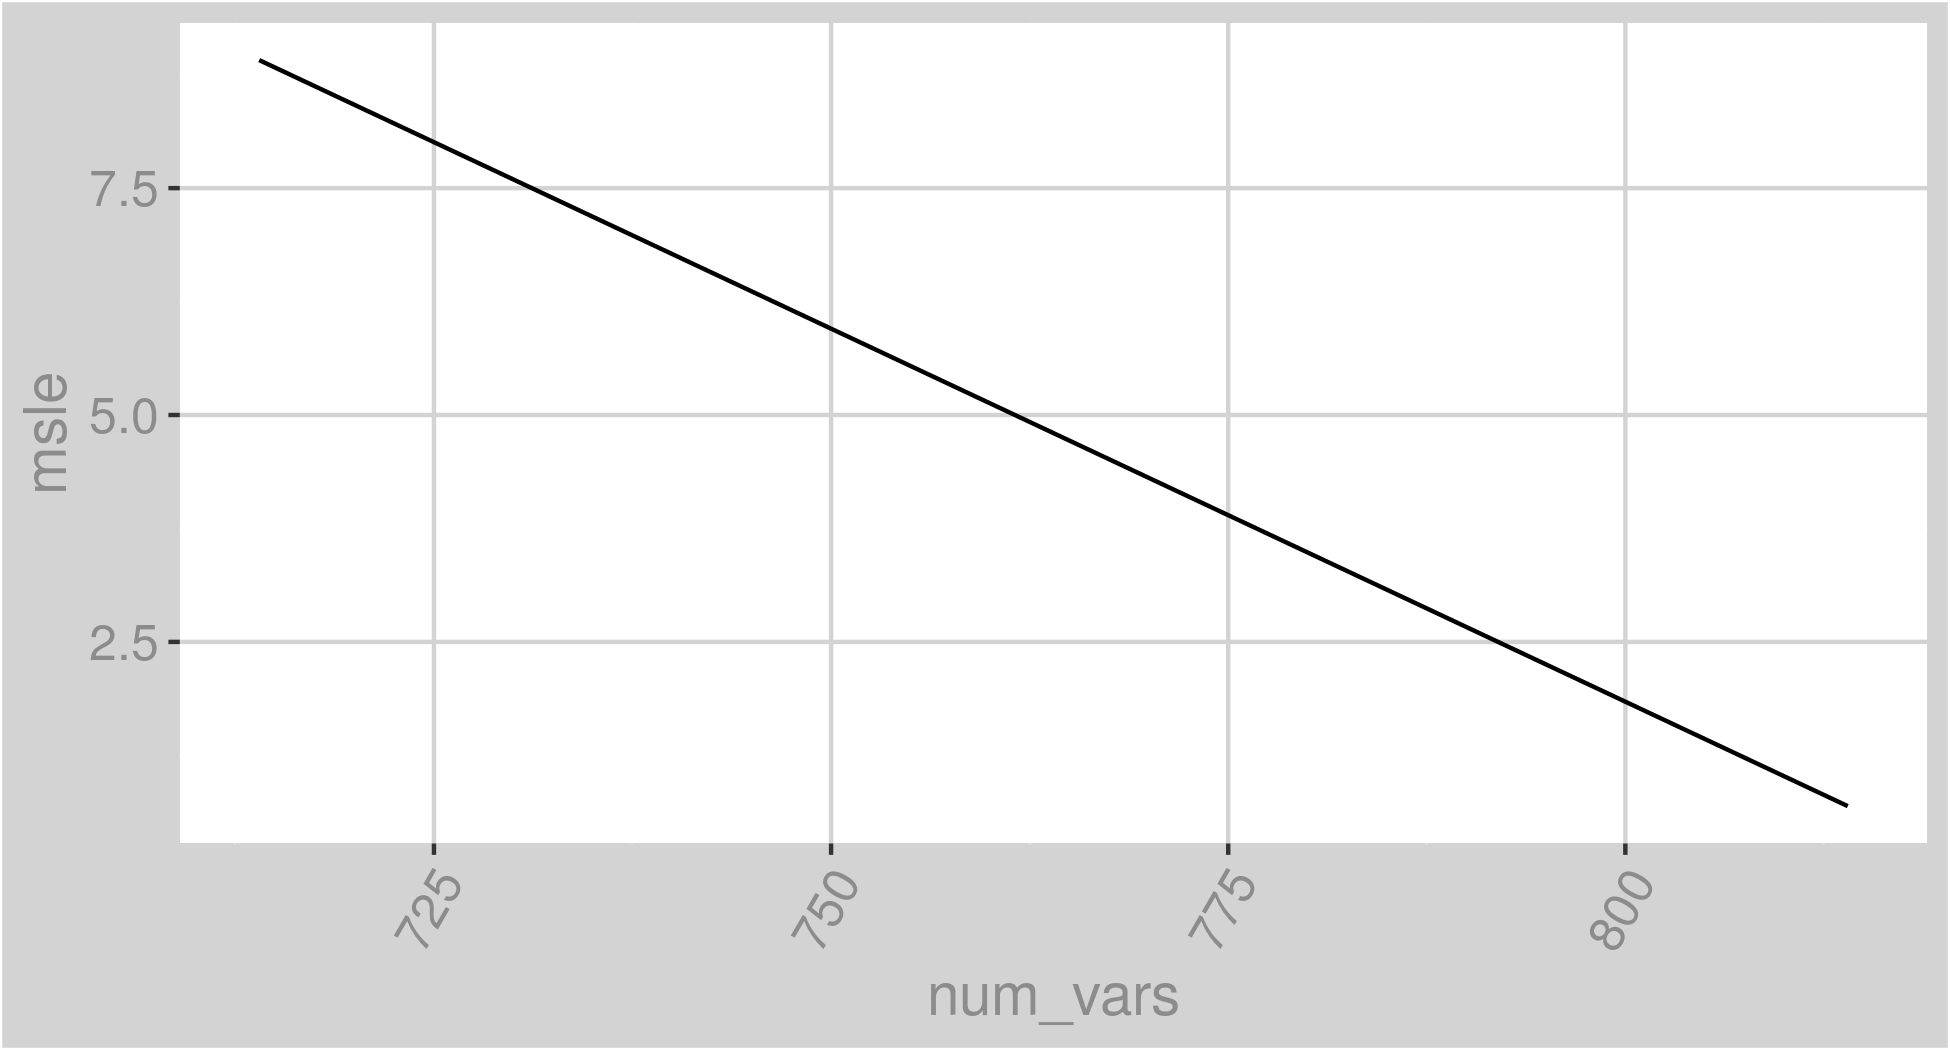
\includegraphics[width=\textwidth, height=0.25\textheight]{Images/electricity_nn_error.png}
\end{figure}

The final selected model, after re-training, has a MSLE of 0.875 and RMSE of 15357.  Comparing this model ('Full Neural Network') to the previous feature extraction models, which used many more variables, the performance is competitive.  Note, in an effort to provide a sufficient number of data points for such a large model, 50\% of the training data had noise added to the numeric columns and appended to the existing set.

\begin{figure}[h]
\centering
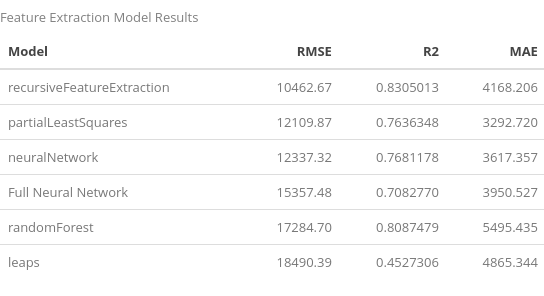
\includegraphics[width=0.6\textwidth, height=0.25\textheight]{Images/electricity_model_summary.png}
\end{figure}

The resdiuals indicate that the variance scales with the response variable; however, since neural network models do not operate on a principle of homoscedacitity, only underlying patterns are of concern. Additionally, the noted error pattern is by design so that higher error in higher consumption projects are acceptable.  \textit{\hyperref[appendix_nn:electricity:nn_full]{Appendix}}

\subsubsection{Variable Selection Summary}
The final model chosen uses 100 variables.  Many of the features within the set have to do with the amount of receptacle equipment within the building as well as major electrical appliances (e.g. elevators) and essential equipment (e.g. data center servers, refrigeration).  In fact, there are only a few cryptic selected variable (e.g. existence of employee breakroom) that may be more related to the building type rather than the actual question being asked.   \textit{\hyperref[appendix_nn:electricity:nn_full_variables]{Appendix}}

\subsubsection{Future Work}
While it was determined that some heteroscedacitity would be acceptable, there does appear to be area for improvement.  Additionally, as mentioned at the beginning of this report, the sampling of this data set was stratified to reflect the building population.  However, it is noted that there are some building classes that have greater variance than others.  Therefore, it may be useful to use this stratification as a weighted method, based on \lstinline{PBAPLUS}, in order to try and emphasize accuracy on the most prevalent budiding types. Also, there was not a lot of attention paid to the actual transformations of the predictors given the large quantity of them.  It is possible a better fit can be obtained with more intelligent transformations applied to the features after further analysis.

The automated selection process does seem to have included some highly correlated pairs, such as requesting the numeric amont of workers as well as the binned category of this value.  This does reduce the number of necessary questions, but it is unclear if both are necessary and/or if they are possibly detrimental.  Also, there are a number of questions that may be automatically known just based on the usage type as some questions do not apply to all buidlings.  It is possible take the steps used in asking questions in the survey in order to build a live form that can automatically parse out the meaningful questions based on building type, which could reduce the need to enter a value for all the selected variables.

\FloatBarrier
\newpage
\subsection{Natural Gas}

\FloatBarrier
\newpage
\subsection{District Heat}

\FloatBarrier
\newpage
\subsection{Fuel Oil}